\section{Results}

\subsection{Datasets and Processing}
\label{data}
In our experiments, we used whole genome sequencing data of two mother-father-child trios I1 (Table \ref{tab:I1}), and G1, published by \cite{kitzman2012}. In our experiments we mainly used the first trio I1 with 13\% fetal admixture in obtained plasma. For maternal, paternal, and plasma datasets the reads were aligned to the hg19 genome using BWA. We genotyped both the parents using Samtools and Vcftools. To improve the precision of genotyping we only consider variants at positions previously identified as variable within the 1000 Genomes Project.  Subsequently we phased the haplotypes using Beagle 4 \citep{browning2013} with reference haplotype panels from 1000 Genomes Project. 
\begin{table}
\caption{Summary of mother-father-child trio I1 sequencing data, courtesy of \cite{kitzman2012}  }
\label{tab:I1}
\centering
\footnotesize
\begin{tabular}{l|l|c}
\hline
Individual & Sample & DOC \\ \hline\hline
Mother (I1-M) & Plasma (5 ml, gestational age 18.5 weeks) & 78 \\
	& Whole blood ($<1$ ml) & 32 \\
Father (I1-P) & Saliva & 39 \\
Child (I1-C) & Cord blood at delivery & 40 \\
\hline
\end{tabular}
\end{table}

\subsection{Evaluation}
\begin{table*}
\caption{Summary of recall on test set composed of 360 \emph{in silico} simulated CNVs in I1 maternal plasma samples with 13\% and 10\% fetal admixture ratio. The `ratios only` column corresponds to the method that only uses allelic ratios, but not the coverage prior. In such cases both the precision and  recall are mostly dominated by the model combining both signals. (We write `NA` in a precision field if no call of such CNV category was predicted by the model)}
\label{tab:resRecall}
\centering
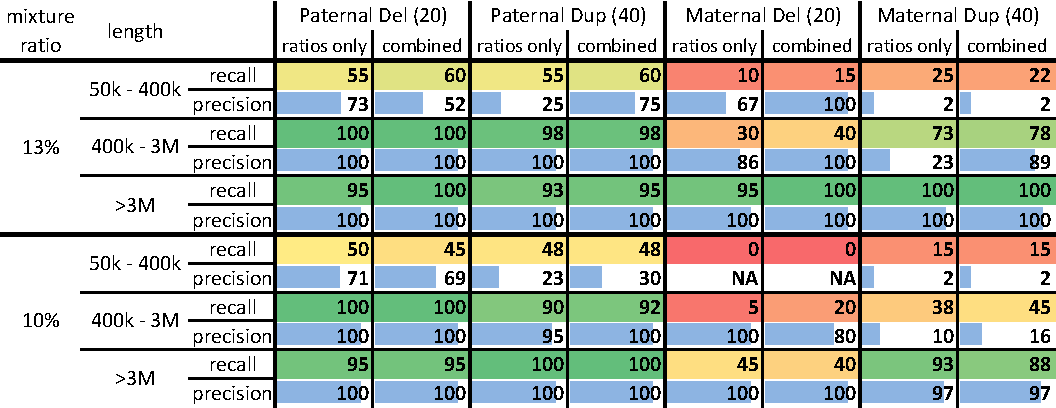
\includegraphics[width=0.85\textwidth]{figures/ismb_res_color}
%\vspace{3pt}
\end{table*}

We simulated 360 CNVs in I1 plasma to evaluate our method's recall, while G1 plasma sample served as a reference in DOC-based CNV estimation as described in Section \ref{ss:coverage}. For each test case, we  picked a random position in chromosome 1, outside known centromere and telomeres regions, to place the simulated CNV.  Our simulation methods are described in detail in Section \ref{ss:simulation}. We then ran our algorithm on a genomic window starting 20Mb before the simulated CNV and ending 20Mb after the CNV. The results are shown in Table \ref{tab:resRecall}. We acknowledge a CNV as correctly called if CNV predictions of the same type span at least 50\% of it, while precision is computed as the fraction of correct CNV calls over all calls of that category. To evaluate the effect the admixture has on accuracy, we repeated this experiment not only with the original plasma dataset, but also once down-sampled to only contain 10\% admixture.

The results indicate that our method can achieve nearly perfect recall and precision for variants ${>3}$ megabases, and promising results down to CNVs of 400 kilobases.  Maternally inherited events are typically more difficult to identify than paternally inherited ones, and deletions more difficult than duplications, possibly due to complete dropout of fetal alleles due to reduced admixture.

\begin{table*}
\caption{Summary of results obtained by an HMM using only WRV signal. The same test set composed of 360 \emph{in silico} simulated CNVs was used as in Table \ref{tab:resRecall}. We ran the model with 100kb, and 300kb bin sizes. (We write `NA` in a precision field if no call of such CNV category was predicted by the model)}
\label{tab:resWRV}
\centering
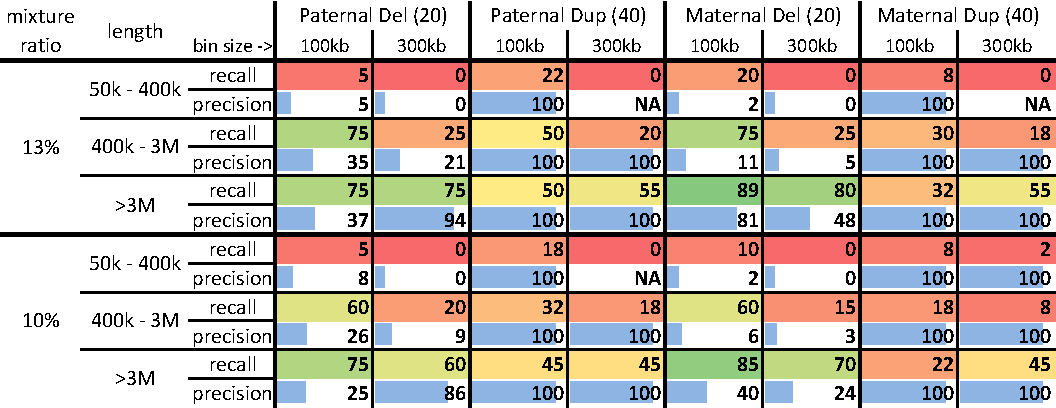
\includegraphics[width=0.85\textwidth]{figures/ismb_wrv_res_color}
\end{table*}

To evaluate power of individual signals utilized by our unified model, we also tested models that take into consideration only either the allelic ratios or coverage information. The allelic ratios only model is as described above in Section \ref{ss:hmm} but without multiplying of copy number prior in the transition probabilities. Obtained results are shown together with the results of the unified model in Table \ref{tab:resRecall}. 

For predicting fetal CNVs based solely on coverage information we split the sample to bins of uniform size and computed WRVs for each, following the work of \cite{srinivasan2013}. We then ran a simple HMM with 3 states corresponding to normal inheritance, duplication, and deletion, respectively. The WRVs in bins were interpreted as emissions and the emission distributions were computed as described in Section \ref{ss:coverage}, Equation \ref{eq:wrv_distrib}. We tested the HMM with bin sizes of 100kb and 300kb, and the results are summarized in Table \ref{tab:resWRV}. Using larger bins limit resolution of the method, e.g. in case of 300kb bins the obtained recall on ${<400}$kb CNVs is (close to) zero. On the other hand for large CNVs ${>3}$Mb using 300kb bin size mostly improves upon 100kb bins in terms of both recall and precision.
%Note that models based solely on coverage information are more sensitive towards deletions than duplications. This is due to stronger coverage signal imposed by a deletion, causing half of the fetal portion to be missing, compared to duplication 

\begin{table*}
\caption{In silico recall and number of CNVs of various sizes generated in a genome-wide run. For each CNV size we also show (in parenthesis) the number of calls that are from at least 50\% overlapped by CNVnator \citep{abyzov2011cnvnator} calls on the fetal, maternal, and paternal genomes, respectively.}
\label{tab:resWGS}
\centering
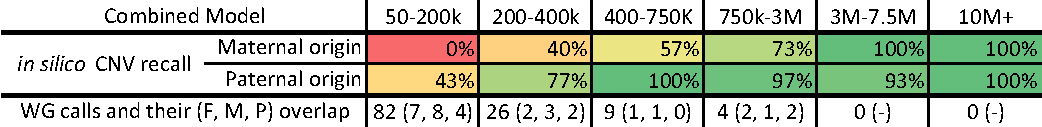
\includegraphics[width=0.78\textwidth]{figures/wg_calls_color}
\end{table*}

To further test precision of our combined method, we ran our combined model on the whole plasma dataset (expected to contain no large de-novo variants) and observed the number of CNV calls for each size. These numbers are shown in Table \ref{tab:resWGS}, with \textit{in silico} accuracy for each length shown for comparison. Notably, a large fraction of the larger false positive calls correspond to CNVs already present in parents (and hence inherited, rather than de novo). 

\subsection{Implementation Note}
Our model is implemented in the Python programming language with the PyPy interpreter. When ran on a 	whole genome dataset our implementation required up to 20GB of system memory and took less than 4 hours of single thread CPU time to finish.
